%Why heterogenous memory systems

%Memory access pattern matching to reduce cost

%Trends in heterogeneous memory systems

%Challenges associated with the trend

%Differences on memory characteristics make MM challenging

%Argue for adoption in production systems


%%%%% BORING INTRO :P %%%%%
%Main memories contribute to $\approx$ 30\% of machine cost (based on assembling
%a server class machine on newegg.com in January 2017). The significant cost of
%main memories make them an important resource that should be utilized
%efficiently to justify their cost contribution. To cater to the memory needs of
%applications from different domains (for example: data-centers, cloud computing,
%supercomputers) exhibiting different memory access patterns, systems are
%becoming heterogeneous to adapt to variations in memory access patterns
%(differnces in bandwidth requirements, latency tolerance) with the aim to reduce
%the cost to run the applications.
%
%The emergence of {\it heterogeneous memory systems} has resulted in a need for
%new memory management policies that are able to fully exploit these systems.
%While traditional memory management techniques largely assume a ``homogeneous''
%main memory, future systems are likely to have two or more different types of
%main memories attached to them -- thus the term ``heterogeneous'' memory
%systems. An example of such a system is the recently announced NVIDIA Pascal
%GPU~\cite{pascal}, which is slated to have a high bandwidth connection to the host
%CPU via NVLink~\cite{NVLINK} and thus can access host memory seamlessly.
%Another example is Intel/Micron's 3-D XPoint technology~\cite{xpoint}, which
%provides a slow but cheaper and large capacity non-volatile memory (NVRAM) along
%with a conventional DRAM memory attached to the same CPU node.
%%%%% BORING INTRO ENDS :) %%%%%

Heterogeneity is ubiquitous in systems ranging from supercomputers, data-centers
to smartphones. Fastest supercomputers in the world are comprised of graphics
processing units (GPUs), Xeon Phi processors alongside central processing units
(CPUs)~\cite{top500nov}. Similarly, data-centers deploy GPUs and field-programmable
gate arrays (FPGA) for accelerating applications like web search and machine
learning~\cite{catapultmicrosoft}. Largest cloud provider Amazon Web Services (AWS) offers
instances with GPUs and FPGAs as well~\cite{awsinstances}, indicating that such
heterogeneous platforms are desirable for running contemporary and future
computing applications.

%Applications having varying memory access patterns and heterogeneous memory
%systems provide an opportunity to match application characteristics with that of
%different memory technologies in a heterogeneous memory system. For example,
%when an embarassingly parallel application like matrix multiplication is run on
%a machine installed with low bandwidth main memory technology, then memory-level
%parallelism (MLP) present in the application is wasted. Due to the mis-match in
%application memory access pattern and memory technology installed on the
%machine, the application will take longer time to finish. Alternatively, if the
%same application runs on a machine installed with high bandwidth memory
%technology then MLP in application can be matched with the higher memory
%bandwidth and thus application can run faster reducing the CPU time needed for
%completion. And this reduction in CPU time implies reduction in cost to run the
%application.  This cost reduction can trickle down to the reduced cost seen by
%the customer either running such applications as a service or paying for such
%services~\cite{AWS-pricing-model}.

Heterogeneous memory systems, though lucrative, pose several challenges on system
design and programmability. Even more so, if such heterogeneous systems are built by
separate vendors like machines with separate graphics cards (e.g., P2 and G2
instances in AWS EC2~\cite{awsinstances}). With a
trend in data-center/cloud applications to map large datasets in memory,
installed memory capacity per machine is rapidly growing~\cite{spark}. The
challenge is to scale existing or formulate new memory management policies that
can manage the rapidly growing memory capacity and also support differences in
characteristics of different memory tecnologies.

%With the advancement of interconnect technologies like NVIDIA
%NVLINK~\cite{}, existing heterogeneous CPU--GPU systems present an opportunity
%to maximize bandwidth available to GPUs from...

Differences in memory charateristics and rapid growth in memory capacity make
memory management of such heterogeneous systems challenging. Decisions about
data placement and movement have to be made in an application transparent manner
while simplifying system design and programmability of already complex
heterogeneous systems. Application transparent policies are desirable as they do
not require any extra effort from the programmer, which enables the adoption of
such policies easier. Simple but effective designs can reduce development and
verification efforts, thus the time to market, enabling easier adoption of
heterogeneous memories in production systems.

Previous academic and commercial systems study Non-Uniform Memory Access~(NUMA)
extensively. The main optimization goal in such NUMA systems was to cut
down on memory access latency as much as possible. However, in domains such as
GPGPU computing or data-centers, characteristics
such as bandwidth or access cost per bit are far more critical. In this thesis, we study memory characteristics
beyond memory access latency with the goal to simplify system design, easing
programmability, while squeezing the best possible performance out
of such heterogeneous memory systems.  Next we briefly discuss key aspects that
are relevant to modern incarnations of heterogeneous memory in GPUs and
data-centers.

\begin{enumerate}
\item
\textbf{Different memory bandwidths:}
Different memory technologies will typically have differences in their
bandwidths, e.g., a GPU connected to on-board GDDR and host-side DDR memories
can have a bandwidth differential of 2 -- 8$\times$ between the two
memory technologies (example systems shown in Figure~\ref{fig:arch-hpca2015}).
Since GPUs are sensitive to main memory bandwidth (due to massive thread-level
parallelism), the metric to optimize in such systems is the total available
bandwidth to the GPU from the two memory sources. While prior work on
Non-Uniform Memory Access has closely looked at data placement strategies
to optimize the total memory {\it access latency} in the presence of different
memory zones with different access latencies, we show that such policies are not
suited to optimizing the total memory {\it bandwidth}. Instead, we propose {\it
Bandwidth-Aware Placement} (BW-AWARE), which directly maximizes the overall
bandwidth, and show that it can significantly increase application throughput
for several GPU applications.

\item
\textbf{Different memory coherency domains:} 
In a heterogeneous CPU--GPU memory system, hardware cache coherence can improve
performance by allowing concurrent, fine-grained access to memory by both CPU
and GPU.  However, implementing hardware cache coherence between the CPU and the
GPU can lead to significant challenges because of design and verification
involved particularly if the two domains are designed by separate vendors. We
introduce {\it Selective Caching}, a coherence policy that disallows GPU caching
of any memory that would require coherence updates to propagate across the two
domains. This approach decouples the cache-coherence protocols in CPUs and GPUs,
thus \fixme{has a potential to improve cross-vendor design cycle time.}

\item
\textbf{Different costs per bit:}
%\fixme{Modify THP stuff and write about application-transparency.}
Different memory technologies can have different monetary costs.  For example,
recently announced non-volatile memory technology~\cite{xpoint} is projected to
be significantly cheaper than regular DRAM, while also being significantly
higher latency. Its lower cost per bit makes it a good candidate for use in
data-centers, where main memory cost can be $\approx$ 30\% of the server machine
cost, translating to $3-15\%$ of the total cost of ownership (TCO), amounting to
bilions of dollars~\cite{borosso2013}. However, \fixme{their} low speed means that only
{\it cold}, i.e., infrequently accessed data can be placed in such memories.
Detection of such cold data \fixme{must} be done {\it application-transparently}, since
that allows cloud providers to transparently swap out slow memory in place of
DRAM.
%However, placing more cold data in the slower memories conflicts with efficient
%virtual memory usage by transparent huge page (THP), which can provide up to
%30\% performance gains in large memory footprint data-center applications as we
%show in Table~\ref{tab:thp-benefit}.
We study how to place as much data in slow memory as possible, while being
completely application-transparent, to improve
performance per dollar in data-centers.  \end{enumerate}

Below, we describe each of these three problems in detail and give a brief
sketch of our proposed solution to these problems.

\section{Bandwidth-asymmetric Systems}
GPU-attached Bandwidth-Optimized (BO) memory (e.g., GDDR5) has been allocated
and managed primarily through explicit, programmer-directed function calls for
obtaining maximum throughput out of GPUs.  To make best use of the bandwidth
available to GPU programs, programmers have to explicity call memory copy
functions to copy the data over the relatively slow PCIe bus to the GPU memory,
and --- only then --- launch their GPU kernels.  This up-front data allocation
and transfer has been necessary since transferring data over the PCIe bus is a
high overhead operation, and a bulk transfer of data amortizes this overhead.
This data manipulation overhead also results in significant porting challenges
when retargeting existing applications to GPUs, particularly for high-level
languages that make use of libraries and dynamic memory allocation during
application execution.

\begin{figure}[t]
    \centering
    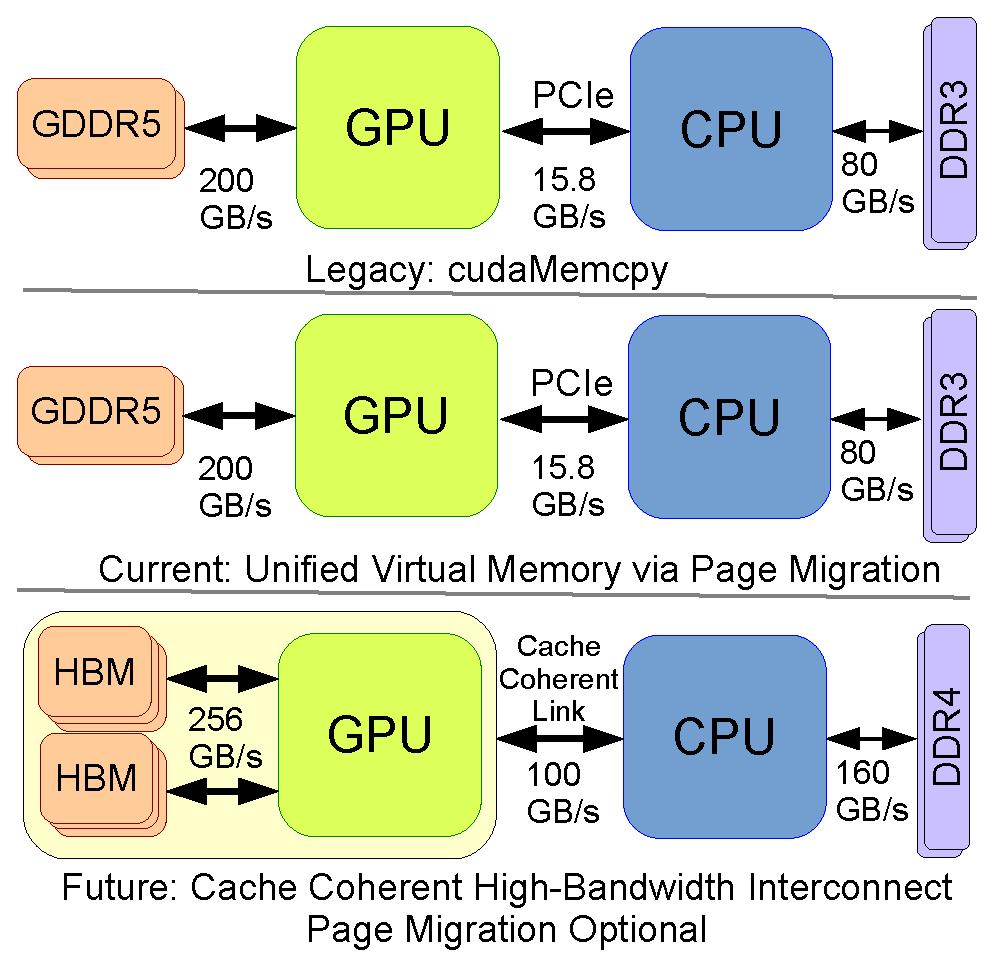
\includegraphics[width=0.7\columnwidth]{hpca2015/figures/architecture.eps}
    \caption{System architectures for legacy, current, and future mixed GPU-CPU systems.}
    \label{fig:arch-hpca2015}
\end{figure}

Recognizing the obstacle programmer-directed programming model poses to the
wider adoption of GPUs in more parallel applications, programming systems like
NVIDIA's CUDA, OpenCL, and OpenACC are evolving to shared virtual address space
between CPU and GPU~\cite{UVM}. With the availability of Unified Virtual Memory
(UVM)~\cite{UVM} for NVIDIA GPUs the programmer-directed manual copy
requirements has been lifted.  Concurrently, CPU--GPU architectures are evolving
to have unified globally addressable memory systems in which both the GPU and
CPU can access any portion of memory at any time, regardless of its physical
location.  Today this unified view of memory is layered on top of legacy
hardware designs by implementing software-based runtimes that dynamically copy
data on demand between the GPU and CPU~\cite{cuda}. \fixme{This} results in significant
throughput degradation as data copy time is not overlapped with GPU kernel
launch latency, resulting in exposure of data copy latency to the GPU kernel run
time. Thus, systems with the highest throughput requirements (i.e., majority of
GPGPU systems) still use programmer-optimized code to run on GPUs.

As depicted in Figure~\ref{fig:arch-hpca2015}, over the next several years it is
expected that GPU and CPU systems will move away from the PCIe interface to a
fully cache coherent (CC) interface ~\cite{AMDHSA}. These systems will provide
high bandwidth ($5-10\times$ higher) and low latency ($10\times$ lower) between
the non-uniform memory access (NUMA) pools attached to discrete processors by
layering coherence protocols on top of physical link technologies such as
NVLink~\cite{NVLINK}, Hypertransport~\cite{AMDHT}, or QPI~\cite{INTELQPI}.

As heterogeneous CPU--GPU systems move to a transparent unified memory system,
the OS and runtime systems need information about other aspects of memory zones
such as their bandwidths instead of only the access latency information that is
exposed today via Advanced Configuration and Power Interface. In CC-NUMA
systems today, latency information alone is adequate as CPUs are generally more
performance sensitive to memory system latency rather than other memory
characteristics. In contrast, massively parallel GPUs and their highly-threaded
programming models have been designed to gracefully handle long memory
latencies, instead demanding high bandwidth. Unfortunately, differences in
bandwidth capabilities, read versus write performance, and access energy are not
exposed to software; making it difficult for the operating system, runtime, or
programmer to make good decisions about memory placement in these GPU-equipped
systems. In this thesis (Chapters~\ref{chap:asplos2015},~\ref{chap:hpca2015}) we
investigate the effect on GPU performance of exposing memory system bandwidth
information to the operating system/runtime and user applications to improve the
quality of dynamic page placement and migration decisions. We propose
Bandwidth-Aware (BW-AWARE) page placement and dynamic page migration to fully
utilize memory bandwith for throughput-oriented CPU--GPU heterogeneous memory
systems~\cite{ref:agarwal:hpca2015,ref:agarwal:asplos2015}.

\section{Different Coherence Domains}
%Technology trends indicate an increasing number of systems designed with CPUs,
%accelerators, and GPUs coupled via high-speed links. Such systems are likely to
%introduce unified shared CPU-GPU memory with shared page tables. In fact, some
%systems already feature such implementations~\cite{AMDKaveri}.
Introducing globally visible shared memory improves programmer productivity by
eliminating explicit copies and memory management overheads. Whereas this
abstraction can be supported using only software page-level protection
mechanisms~\cite{UVM, HSA}, hardware cache coherence can improve performance by
allowing concurrent, fine-grained access to memory by both CPU and GPU.
%If the CPU and GPU have separate physical memories, page migration may also be
%used to optimize page placement for latency or bandwidth by using both near and
%far memory~\cite{Dashti2013,Agarwal2015b,Meswani2015,Chou2015}.

%Some CPU--GPU systems will be tightly integrated into a system on chip (SoC)
%making on-chip hardware coherence a natural fit, possibly even by sharing a
%portion of the on-chip cache hierarchy~\cite{HSA,AMDAPU,Hechtman2014}.  However,
%the largest GPU implementations consume nearly 8B transistors and have their own
%specialized memory systems~\cite{NVIDIA8BILLION}.  Power and thermal constraints
%preclude single-die integration of such designs.  Thus, many CPU--GPU systems
%are likely to have discrete CPUs and GPUs connected via dedicated off-chip
%interconnects like NVLINK (NVIDIA), CAPI (IBM), HT (AMD), and QPI (INTEL) or
%implemented as multi-chip modules~\cite{NVLINK,CAPI,AMDHT,INTELQPI,Chen92}.
%The availability of these high speed off-chip interconnects has led both
%academic groups and vendors like NVIDIA to investigate how future GPUs may
%integrate into existing OS controlled unified shared memory regimes used by
%CPUs~\cite{Pichai2014,Power2014,Agarwal2015,Agarwal2015b}.

Despite the programmability benefits of CPU--GPU cache coherence, designing such
a system can pose several hurdles. Prior
studies~\cite{Hong2012,Vantrease:2011:ACL:2014698.2014902} have shown
that coherence implementations are a major source of hardware design bugs.
Extending a CPU coherence implementation to a GPU over a long-latency
interconnect ($\approx$ 100ns)  will only increase the design cost of such a
system.  Also, if the CPUs and GPUs are to be manufactured by different vendors,
a high level of coordination is needed between those two vendors --
including coordination on the specification of coherence implementation and
verification efforts. Quoting George Bernard Shaw:

\begin{centering}
\textit{``The single biggest problem in communication is the illusion it has already
taken place.''}
\end{centering}
Such hurdles make CPU--GPU cache coherence an unattractive option to
deploy in a product.

Current CPUs have up to 18 cores per socket~\cite{INTELXEONE5V3} but GPUs are
expected to have hundreds of streaming multiprocessors (SMs) each with its own
cache(s) within the next few years. Hence, extending traditional hardware
cache-coherency into a multi-chip CPU--GPU memory system requires coherence
messages to be exchanged not just within the GPU but over the CPU--GPU
interconnect. Keeping these hundreds of caches coherent with a traditional HW
coherence protocol, as shown in Figure~\ref{fig:motivation}, potentially
requires large state and interconnect bandwidth~\cite{Kelm2010,johnson2011}.
Some recent proposals call for data-race-free GPU programming models, which
allow relaxed or scoped memory consistency to reduce the frequency or hide the
latency of enforcing coherence~\cite{Hechtman2014}.  However, irrespective of
memory ordering requirements, such approaches still rely on hardware
cache-coherence mechanisms to  avoid the need for software to explicitly track
and flush modified cache lines to an appropriate scope at each synchronization
point. Techniques like region coherence~\cite{Power2013} seek to scale coherence
protocols for heterogeneous systems, but require pervasive changes throughout
the CPU and GPU memory systems.  Such approaches also incur highly coordinated
design and verification effort by both CPU and GPU vendors~\cite{Hong2012} that
is challenging when multiple vendors wish to integrate existing CPU and GPU
designs in a timely manner.

Due to the significant challenges associated with building such cache-coherent
systems, in this thesis (Chapter~\ref{chap:hpca2016}), we architect a GPU
\textit{selective caching} mechanism~\cite{ref:agarwal:hpca2016}.  This
mechanism provides the conceptual simplicity of CPU--GPU hardware cache coherence
and maintains a high level of GPU performance (93\% of hardware cache-coherent
system), but does not actually implement complex hardware cache coherence
between the CPU and GPU.
%In our proposed selective caching GPU, the GPU does not cache data that resides
%in CPU physical memory, nor does it cache data that resides in the GPU memory
%that is actively in-use by the CPU on-chip caches.  This approach is orthogonal
%to the memory consistency model and leverages the latency tolerant nature of
%GPU architectures combined with upcoming low-latency and high-bandwidth
%interconnects to enable the benefits of shared memory.

\section{Cheaper Memory Technologies}
Upcoming memory technologies, such as Intel/Micron's recently-announced 3D
XPoint memory~\cite{3dcrosspoint}, are projected to be denser and cheaper per
bit than DRAM while providing the byte-addressable load-store interface of
conventional main memory.  Improved capacity and cost per bit come at the price
of higher access latency, projected to fall somewhere in the range of 400ns to
several microseconds~\cite{3dcrosspoint} as opposed to 50--100ns for DRAM.  Slow
memory can result in a net cost win if the cost savings of replaced DRAM
outweigh the cost increase due to reduced program performance or by enabling a
higher peak memory capacity per server than is economically viable with DRAM
alone.

However, deploying such memories in a cloud service for use by its customers is
riddled with several challenges. It is important for cloud providers to be able
to provide service-level-agreements (SLAs) to customers guaranteeing performance
of the cloud platform. To provide such SLAs in the presence of slow memory, any
memory placement policy must estimate the performance degradation associated
with placing a given memory page in slow memory, which in turn requires some
method to gauge the {\it page access rate}. Lack of accurate \textit{and}
performant page access rate tracking in contemporary x86 hardware makes this
task challenging.

Making slow memory use application-transparent is particularly critical for
cloud computing environments, where the cloud provider may wish to transparently
substitute cheap memory for DRAM to reduce provisioning cost, but has limited
visibility and control of customer applications.  Relatively few cloud customers
are likely to take advantage of cheaper-but-slower memory technology if they
must redesign their applications to explicitly allocate and manage hot and cold
memory footprints. A host-OS-based cold memory detection and placement mechanism
is a natural candidate for such an environment.

In this thesis (Chapter~\ref{chap:thermostat}) we propose {\it
Thermostat}~\cite{ref:agarwal:asplos2017:thermostat} that manages two-tiered
main memory transparently to applications while preserving the benefits of huge
pages and dynamically enforcing limits on performance degradation (e.g.,
limiting slowdown to 3\%).

%%It's an unsolved problem
%Prior academic work on two-tiered memory has assumed migration/paging at 4KB
%page granularity.  Huge pages, implemented via Linux's Transparent Huge Page
%(THP) mechanism, are now ubiquitous and critical for data-center applications,
%boosting application performance by 10-15\%.
%%Recent work~\cite{JeffPaper} has demonstrated that 2MB huge pages are particularly
%%performance-critical under virtualization.  
%%For example, our study demonstrates a 20\% throughput improvement for Hadoop and
%%a 40\% speedup on random memory probes when using huge pages under
%%virtualization.  
%However, huge pages thwart prior two-tiered memory proposals for two reasons:
%(1) it is too expensive to frequently migrate pages at 2MB granularity, and (2)
%hot regions occur within otherwise cold 2MB huge pages can hurt performance if
%placed in the slower memory. 
%
%%Here is my idea
%We propose to develop a transparent huge-page-aware two-tiered memory solution
%that integrates support for dynamic page migration and transparent huge pages,
%achieving both the capacity/cost advantages of two-tiered memory and performance
%advantages of huge pages.  Our focus is on cloud computing scenarios where a
%high-memory-footprint application, such as Cassandra, Aerospike, or MySQL, runs
%under virtualization and may co-run with other, competing applications.  Hot
%regions within otherwise cold huge pages present a central challenge to our
%objective; existing x86-Linux provides no mechanism to carve out a 4KB hot
%region within a 2MB cold page.
%
%%So, we propose translation facades, a 4KB
%%translation that remaps a portion of a 2MB mapping with an alternate physical
%%address or permissions.  Current x86-Linux requires non-overlapping mappings due
%%to hard-coded page table structure and because TLB entries are replaced
%%independently, hence, an uncached 4KB facade to a cached 2MB translation could
%%lead to a mis-translation. We will pursue implementations of translation
%%facades along two paths. (1) Hardware support: we will extend x86 page table and
%%TLB design to support facades. (2) Virtualization: Our existing study of huge
%%pages under virtualization demonstrate that a majority of the benefit can be
%%obtained if host pages are 2MB even if guest pages are 4KB.  We will investigate
%%if the two-level translation from guest to host to machine addresses can be
%%exploited to emulate hardware support for translation facades.
%
%%Bulleted list of contributions
%We propose to develop a Linux prototype that will to estimate the properties of
%a system with the following properties:
%
%\begin{enumerate}
%\item
%We will measure hot and cold memory fractions at 4KB granularity and within 2MB
%huge pages to measure two-tiered memory opportunity. We will use kstaled (an
%optional extension to the Linux kernel that tracks pages that have not been
%accessed over a fixed time interval) and BadgerTrap~\cite{ref:badgertrap} (a tool to
%intercept TLB misses in software) to facilitate this characterization. 
%
%\item
%We will develop methods to track hot and cold memory regions at run-time.  A
%key challenge lies in efficiently tracking hot regions within an otherwise-cold
%huge page, as kstaled provides visibility only at page granularity.  We propose
%to investigate sampling methods, e.g., by probabilistically demoting huge pages
%or leveraging performance counter infrastructure. 
%
%\item
%We will develop an online migration mechanism that can shift data between
%fast and slow memory tiers while the application is concurrently executing.  We
%draw experience from existing NUMA migration and THP memory defragmentation. We
%will implement the migration mechanism in the Linux kernel.
%
%\item
%We will develop translation facades, a mechanism that remaps a
%portion of a 2MB mapping with an alternate physical address or permissions
%(using BadgerTrap to emulate performance) and investigate novel page table and
%TLB organizations to support facades.
%\end{enumerate}

\section{Contributions}
In this thesis we make following contributions:

\begin{itemize}
\item
We show that existing CPU-oriented page placement policies are not only 
sub-optimal for placement in GPU-based systems, but simply do not have the 
appropriate information available to make informed decisions when optimizing for 
bandwidth-asymmetric memory systems. Exposing additional bandwidth information 
to the OS, as is done for latency today, will be required for optimized decision 
making. (Chapter~\ref{chap:asplos2015})

\item
We show that placing all pages in the bandwidth optimized memory is not the best
performing page placement policy for GPU workloads.  We propose a new
bandwidth-aware (BW-AWARE) page placement policy that can outperform Linux's
current bandwidth-optimized INTERLEAVE placement by 35\% and the default latency
optimized LOCAL allocation policy by as much as 18\%, when the application
footprint fits within bandwidth-optimized memory capacity.
(Chapter~\ref{chap:asplos2015})

%\item
%For \emph{memory capacity constrained} systems (i.e. bandwidth-optimized memory
%capacity is insufficient for the workload footprint), we demonstrate that using
%simple application annotations to inform the OS/runtime of hot versus cold data
%structures can outperform the current Linux INTERLEAVE and LOCAL page placement
%policies.  Our annotation based policy combined with bandwidth information can
%outperform these page placement policies by 19\% and 12\% respectively, and get
%within 90\% of oracle page placement performance.

\item
We show that counter-based metrics to determine when to migrate pages from the
CPU to GPU are insufficient for finding an optimal migration policy to exploit
GPU memory bandwidth.  In streaming workloads, where each page may be accessed
only a few times, waiting for $N$ accesses to occur before migrating a page will
actually limit the number of accesses that occur after migration, reducing the
efficacy of the page migration operation. (Chapter~\ref{chap:hpca2015})

%\item
%TLB shootdown and refill overhead can significantly degrade the performance of
%any page migration policy for GPUs\@. We show that combining reactive migration
%with virtual address locality information to aggressively prefetch pages can
%mitigate much of this overhead, resulting in increased GPU throughput (35\%).

%\item
%The legacy intuition to migrate all data to the GPU local memory in an attempt
%to maximize bandwidth fails to leverage the bandwidth available via the new
%CC-NUMA interface.  A page migration policy which is aware of this differential
%and balances migration with CC-NUMA link utilization will outperform either GPU
%or GPU memory being used in isolation.

\item 
We present a software based memory migration system that, on average,
outperforms CC-NUMA based accesses by 1.95$\times$, performs 6\% better than the
legacy CPU to GPU {\tt memcpy} approach by intelligently using both CPU and GPU
memory bandwidth, and comes within 28\% of oracular page placement, all while
maintaining the relaxed memory semantics of modern GPUs.
(Chpater~\ref{chap:hpca2015})

%\vspace{-.025in}
\item
We propose GPU selective caching, which can provide a CPU--GPU system that
provides a unified shared memory without requiring hardware cache-coherence
protocols within the GPU or between CPU and GPU caches.
We identify that much of the improvement from GPU caches is due to coalescing 
memory accesses that are spatially contiguous within a cache line.  Leveraging
aggressive request coalescing, GPUs can achieve much of the performance benefit
of caching (80\%), without caches. (Chapter~\ref{chap:hpca2016})

\item
We propose a small on-die CPU cache specifically to handle uncached requests
that will be issued at sub-cache line granularity from the GPU. This cache helps
both shield the CPU memory system from the bandwidth hungry GPU and supports
improved CPU--GPU interconnect efficiency by implementing variable-sized
transfer granularity. (Chapter~\ref{chap:hpca2016})

\item
We demonstrate that a large fraction (60\%) of GPU-accessed data is read-only.
Allowing the GPU to cache this data and relying on page protection mechanisms
rather than hardware coherence to ensure correctness closes the performance gap
between a selective caching and hardware cache-coherent GPU for many
applications. (Chapter~\ref{chap:hpca2016})

\item
We propose Thermostat, an online low-overhead application-transparent page
management mechanism for estimating the performance degradation due to placing a
particular page in slow memory for two-tiered main memory system.  We use this
mechanism in an online, huge-page-aware hot/cold page classification system that
{\it only} requires a target maximum tolerable slowdown as input.
(Chapter~\ref{chap:thermostat})

\item
We propose an online method to detect mis-classifications and rectify them,
thereby minimizing the impact of such mis-classifications on application
throughput.  By emulating slow memory in software, we demonstrate that
Thermostat can migrate up to 50\% of cloud application footprints to slow memory
with a 3\% slowdown, reducing memory provisioning cost up to 30\%.
(Chapter~\ref{chap:thermostat})
\end{itemize}

\section{Impact}
Simple but effective page management algorithms have enormous \fixme{durability}, with no
major changes to locality based page placement occurring in the last several
decades. With the introduction of high bandwidth memory, heterogeneous memory
CPU + GPU systems started shipping in 2016, yet operating systems today are ill
prepared to take advantage of performance-asymmetric memories. As these systems
proliferate, OS page placement policies must fundamentally be re-architected to
account for the underlying topology and technology differences that will be
present in many, if not most, memory systems. While latency-bound applications
(typically run on the CPU) will likely continue to use locality (and thus
latency) to drive their page placement decisions, bandwidth-bound applications
(like GPU workloads) cannot maximize performance without the introduction of new
BW-AWARE page placement algorithms. Similarly, without appropriate page
placement strategies the energy efficiency opportunities presented by
heterogeneous memories will not be realized.

%\textbf{Complexity Reduction OS based Data Management:}
%While there can be notable advantages to using high bandwidth memory as a fine
%grained hardware caching solution, these proposals come with significant down-
%sides, namely implementation complexity. This design burden is further
%compounded when systems are composed of CPUs and GPUs that are not produced by
%a single vendor, or by a single design group within just one company. Operating
%system page placement is the defacto standard for controlling memory utilization
%in multi-processor systems because it effectively decouples the design of
%hardware implementations from runtime memory management, resulting in faster and
%more flexible system development.

BW-AWARE page placement and application aware page placement works seamlessly
across systems where bandwidth ratios vary from $1–1$ up to $1–N$ because the
underlying operating system and runtime environment actively query the available
bandwidth of hardware at execution time. Alternatively, approaches like hardware
DRAM cache approaches are fixed at runtime and optimal cache design is typically
a function of cache capacity to backing memory capacity as well as the relative
bandwidths between the high bandwidth cache memory and backing memory bandwidth.
This combination of conceptual and design simplicity makes operating system page
placement likely to be used in all but the most hardened system designs,
cementing its place as the standard management policy for heterogeneous
memories, for many years to come.

%\textbf{First Practical Approach:} Selective Caching is first practical approach
%to provide a unified, coherent CPU--GPU address space without requiring hardware
%cache coherence, with a potential to enable an explosion in algorithms that leverage tightly
%coupled CPU--GPU coordination.  A major roadblock to fine-grained computation
%sharing between CPU and GPUs today is the absence of a unified, cache-coherent
%shared memory. Due to this shortcoming, extra $cudaMemcpy$ calls have to be added
%in explicitly by the programmer, or the runtime system has to orchestrate bulk
%data transfers between the two devices. This memory management is cumbersome
%and leads programmers to offload computation to GPUs or other accelerators only
%at coarse granularity.  Alternatively, programmers resort to using heavyweight
%runtime systems that manually page memory between the CPU and GPU, at
%considerable performance overhead. These impediments hinder programmer
%productivity.

\textbf{Progammability with Performance:} Whereas cache-coherent access
can boost programmer productivity significantly, it is difficult to implement
cache coherent memory for discrete GPU systems, particularly when the CPU and
GPU are supplied by different vendors (e.g., NVIDIA GPUs in IBM Power servers).
%Despite proposals, there are no generally supported industry standards for
%CPU--GPU hardware cache coherence, and bugs in coherence implementations are
%often due to subtle interactions that are difficult to get right without close
%interaction among implementation teams. Vendor-specific proprietary protocols
%hamper widespread product adoption.
%
%\fixme{compress following para and merge with previous}
Selective caching eliminates the need for a unified hardware cache
coherence protocol, removing the most difficult aspect of providing a unified
shared memory implementation. We see selective caching occupying a feasibility
sweet spot; sacrificing a small amount of performance for enormous wins in
conceptual and implementation complexity.
%Selective caching + request
%coalescing (which provides 80\% of the performance of a hypothetical hardware
%cache-coherent system) requires no coherence coordination between the CPU and
%GPU vendors. Client-side caching calls for a straight-forward addition to the
%CPU design that can enable higher performance unified shared memory abstraction
%for a wide variety of third-party accelerators, in addition to GPUs. Again, the
%implementation choice of the CPU vendor is fully decoupled from a GPU vendor.

%\fixme{Merge time-to-market and Industry impact}
\textbf{Verification and Time-to-market:} Verification is a major factor in the total
cost and time-to-market to ship a processor. CPU--GPU coherence increases
verification overhead significantly, since it requires a combined validation of
the CPU and GPU designs. Debugging problems are particularly difficult in
multi-vendor collaborations, because each vendor is incentivized to reveal as
little of their intellectual property as possible to their counterparts to
preserve market advantage. Selective caching simplifies such collaborations by
removing tight technical entanglements between designs, which can significantly
reduce the time-to-market of new products.

%\textbf{Potential for Follow-on Research:} The possibility of having
%fine-grained sharing among CPUs and GPUs opens up a new area of research into
%applications that exploit finegrain CPU--GPU sharing. The dearth of
%applications that share computation between CPU and GPU at fine granularity is
%due to the fact that there is currently no way to develop and evaluate such
%software. However, the opportunity to partition latency- and bandwidth-sensitive
%computations across CPU and GPU is compelling. By providing a quick path to the
%implementation of unified shared memory, we foresee a host of new programming
%patterns that exploit this capability. Once such programs become commonplace,
%the CPU--GPU coherence interface can then be refined more to cater to the demands
%of such applications.
%
%\textbf{Application Beyond GPUs:} Selective caching is likely to impact
%coherence implementations in other upcoming accelerators as well. Accelerators
%can disallow caching of any CPU data and implement request coalescing to reach a
%competitive CPU-coherent baseline. The simplicity of this baseline means that
%many future accelerators are likely to share a unified memory abstraction,
%thus making programming these accelerators significantly simpler.
%
%\textbf{Industry Impact:}
Because it is difficult to quantify, design simplicity
is rarely a focus of academic research. Yet, we argue that hidden complexities,
such a validation efforts or the requirement for industry wide coordination are
often key impediments that prevents practical adoption of otherwise laudable
academic proposals.
%In this work we specifically seek to slash design complexity
%and reduce the coupling of system components, without sacrificing performance or
%loss of generality. As such, we see innovations like selective caching as
%disproportionately likely to impact industrial practice.
We have partnered with
product groups both within NVIDIA and IBM while pursuing this research to ensure
that practical implementation concerns are first and foremost throughout our
research~\cite{coral2014}.

\textbf{Cheaper Memory Technology in Cloud Deployments:} Slower but cheaper
memory technologies such as NVRAMs hold great promise to lower the memory costs
for cloud vendors. However, vendors have little control over the client
applications, and have to guarantee Service Level Agreements. Also, dependence
on hardware features only delays the adoption of such technologies due to the
time required for rolling out new features in CPUs. Thermostat is the first
policy to our knowledge that addresses these challenges by a software-only
mechanism, thus paving the way towards large-scale deployments of such
technologies in datacenters.

Also, Thermostat's novel software-only sampling policy shows the potential for
using software-only mechanisms for inferring application memory patterns in
runtime at extremely low overhead ($<$ 1\%). We expect that Thermostat's
sampling policy can be employed in other scenarios that require runtime
monitoring of application access patterns, such as resource sharing between
applications, memory access profile-guided optimizations etc.
